\documentclass[11pt,a4paper]{article}
\usepackage[margin=2.5cm]{geometry}
\usepackage[T1]{fontenc}
\usepackage[utf8]{inputenc}
\usepackage{lmodern,microtype,booktabs,longtable,array,graphicx,tikz,hyperref,amsmath,amssymb,float,pdflscape}
\usetikzlibrary{positioning,arrows.meta}
\hypersetup{colorlinks=true,linkcolor=blue!50!black,citecolor=blue!50!black,urlcolor=blue!50!black}
\newcommand{\nN}{93}
\newcommand{\npeer}{57}
\newcommand{\npre}{36}
\newcommand{\nthfednas}{32}
\newcommand{\nthevomoo}{24}
\newcommand{\nthselection}{37}
\newcommand{\nnas}{32}
\newcommand{\nnasevo}{11}
\newcommand{\nnassuper}{10}
\newcommand{\nnaspers}{9}
\newcommand{\nnasres}{23}
\newcommand{\nnasnoniid}{24}
\newcommand{\nnasmoo}{6}
\newcommand{\nnassel}{5}
\newcommand{\nnasfair}{2}
\newcommand{\nnassim}{0}
\newcommand{\nnasevosel}{1}
\newcommand{\nevosel}{12}
\newcommand{\nmoosel}{12}
\newcommand{\nseltotal}{54}
\newcommand{\nselsim}{28}
\newcommand{\nselfair}{15}
\newcommand{\nrlsel}{5}
\newcommand{\nyearmin}{2020}
\newcommand{\nrecent}{54}
\newcommand{\precordsidentified}{1400}
\newcommand{\puniqueopenalexids}{1182}
\newcommand{\paftertitlededup}{1167}
\newcommand{\pafterfederatedabstractfilter}{737}
\newcommand{\paftertopicalfilter}{261}


\title{Evolutionary Neural Architecture Search and Participant Selection\\in Non-IID Federated Learning:\\A Systematic Review}
\author{EvoFederated project\thanks{Single-reviewer, tool-assisted review; see Section~\ref{sec:threats}.}}
\date{Search executed 18 October 2026}

\begin{document}
\maketitle

\begin{abstract}
\noindent\textbf{Background.} Federated neural architecture search (FedNAS), evolutionary and multi-objective optimisation in federated learning (FL), and participant (client) selection under non-IID data have grown largely as separate literatures. \textbf{Objective.} We map how these three lines intersect, with emphasis on (i) searching for a single globally shared architecture, (ii) reducing evaluation cost by training candidates on a subset of clients, and (iii) objectives that capture worst-client behaviour. \textbf{Methods.} We searched OpenAlex with seven pre-specified Boolean queries (publications from 2019 onwards), screened \pafterfederatedabstractfilter{} federated records by rule and \paftertopicalfilter{} candidates by title and abstract, and included \nN{} records (\npeer{} peer-reviewed, \npre{} preprints). \textbf{Findings.} FedNAS work is dominated by supernet/weight-sharing, personalised and resource-aware designs; evolutionary search appears in only \nnasevo{} of \nnas{} NAS records. Evolutionary and many-objective methods are used mostly to choose clients \emph{per training round} or to tune FL hyper-parameters. Similarity-, divergence- and cluster-based selection (\nselsim{} records) targets training convergence, not the cost of candidate evaluation in NAS. We found no included record whose abstract combines architecture search, similarity- or dissimilarity-informed choice of the clients used to evaluate each candidate, and a worst-client objective (one record clusters clients to parallelise a supernet search and another matches label distributions of evaluation groups). \textbf{Full-text appraisal.} Thirteen closest studies were read in targeted fashion: repeated runs are reported by a minority, validation/test discipline varies (some pool validation or test data at the server), mild heterogeneity dominates, and no empirical section reports hypervolume or a worst-client metric. \textbf{Limitations.} One database, one reviewer, abstract-level screening (full-text extraction for 13 studies only); the conclusions about gaps are therefore indicative, not exhaustive.
\end{abstract}

\section{Introduction}
Federated learning trains a shared model without centralising client data \cite{mcmahan2017fedavg}, but statistical heterogeneity makes optimisation and evaluation difficult \cite{kairouz2021advances}. Neural architecture search (NAS) adds an outer loop in which many candidate networks must each be trained, so the number of clients used per candidate becomes a direct cost lever. Three bodies of work are relevant: FedNAS \cite{zhu2021from}; evolutionary and multi-objective optimisation in FL \cite{hartmann2025multiobjective}; and participant selection under non-IID data \cite{smestad2023a}. Evolutionary multi-objective algorithms such as NSGA-II \cite{deb2002nsga2}, NSGA-III \cite{deb2014nsga3} and MOEA/D \cite{zhang2007moead} are the standard tools for the second.

This review addresses four research questions.
\begin{description}
\item[RQ1] How is NAS organised in FL (search paradigm, target model, heterogeneity handled)?
\item[RQ2] Where are evolutionary and multi-/many-objective methods applied in FL?
\item[RQ3] How do similarity, divergence and clustering signals drive participant selection, and for which purpose?
\item[RQ4] Do existing studies combine these elements, and do they use worst-client or fairness objectives and report evaluation cost explicitly?
\end{description}

\section{Methods}\label{sec:methods}
The protocol follows the PRISMA 2020 reporting structure (identification, screening, inclusion); deviations are stated explicitly because the review is automated at the retrieval stage and single-reviewer at the screening stage.

\subsection{Information source and search}
We queried the OpenAlex works endpoint (\texttt{search/search\_openalex.py}) on 18 October 2026. Each of seven queries returned its top 200 records by relevance (two pages of 100), restricted to publications from 1 January 2019 onward and to articles, preprints, book chapters, proceedings articles and reviews. Table~\ref{tab:queries} lists the strings. Hit counts are the totals reported by OpenAlex; only the top 200 per query were retrieved, which is a deliberate depth limit (Section~\ref{sec:threats}).

\begin{table}[H]\centering\small
\caption{Search strings (OpenAlex full-text search syntax).}\label{tab:queries}
\begin{tabular}{p{0.07\linewidth}p{0.68\linewidth}rr}\toprule
ID & String & Hits & Retr.\\\midrule
Q1 & \texttt{"federated neural architecture search"} & 238 & 200\\
Q2 & \texttt{federated AND (evolutionary OR "genetic algorithm" OR NSGA) AND "architecture search"} & 1\,116 & 200\\
Q3 & \texttt{federated learning AND (multi-objective OR multiobjective OR many-objective) AND (evolutionary OR Pareto)} & 5\,890 & 200\\
Q4 & \texttt{("client selection" OR "participant selection") AND "federated learning" AND (heterogeneous OR "non-IID")} & 3\,581 & 200\\
Q5 & \texttt{("client clustering" OR "gradient similarity" OR "update similarity" OR "cosine similarity") AND "federated learning" AND (selection OR clustering)} & 4\,254 & 200\\
Q6 & \texttt{("neural architecture search" OR hyperparameter) AND federated AND (cost OR efficient OR "partial evaluation" OR "low-fidelity")} & 28\,262 & 200\\
Q7 & \texttt{"federated learning" AND (fairness OR "worst-client" OR "worst-case" OR minimax) AND (noniid OR "non-IID" OR heterogeneity)} & 14\,381 & 200\\\bottomrule
\end{tabular}\end{table}

\subsection{Eligibility, screening and coding}
\textbf{Inclusion:} the record (a) concerns federated learning, and (b) addresses at least one of FedNAS/hyper-parameter search, evolutionary or multi-objective optimisation in FL, participant/client selection or clustering under heterogeneity, or is a survey of these. \textbf{Exclusion:} no abstract available; FL only as application context without a methodological contribution on (b); version duplicates (arXiv version of an included article). Screening had three stages: (1) deduplication by normalised title; (2) automatic filters (mentions ``federated''; has an abstract; keyword-defined topical relevance, \texttt{search/screen.py}); (3) manual title/abstract screening of the \paftertopicalfilter{} remaining candidates (\texttt{search/include.py}). Included records were coded \emph{from title and abstract only} with keyword rules (\texttt{search/build.py}) for: NAS, evolutionary/swarm, multi-objective, supernet/weight-sharing, personalisation, resource-awareness, non-IID, client selection/sampling, similarity/clustering/divergence, and fairness/worst-client. Where a count supports a conclusion below, the underlying records were inspected manually; keyword counts are otherwise approximate. Because screening used abstracts (full texts were extracted for 13 studies, Section~\ref{sec:fulltext}), no formal risk-of-bias instrument (Cochrane, Newcastle--Ottawa) was applicable; we report only publication status (peer-reviewed article versus preprint). Metadata of all peer-reviewed records with a Crossref DOI were checked against Crossref (all titles matched); preprints rely on OpenAlex metadata.

\begin{figure}[H]\centering
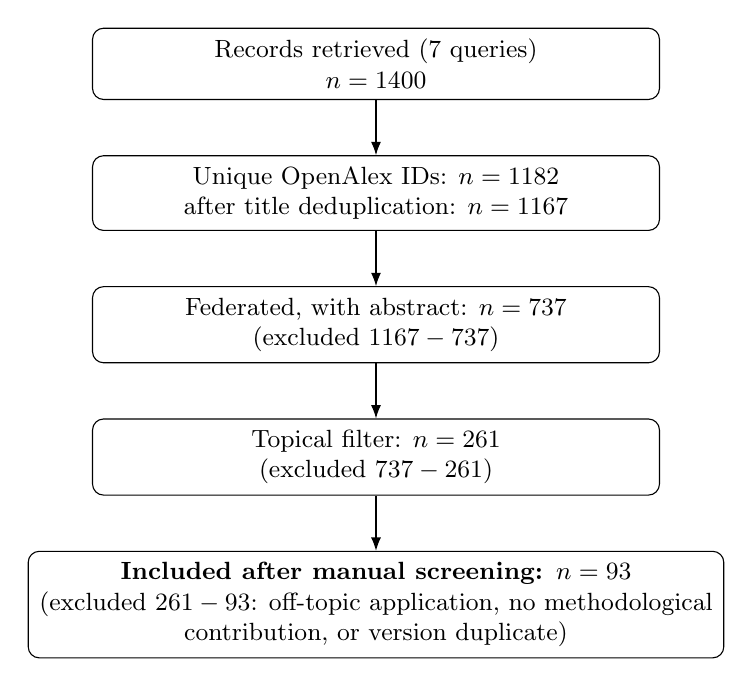
\begin{tikzpicture}[node distance=7mm, box/.style={draw,rounded corners,align=center,minimum width=7.2cm,font=\small,inner sep=4pt}, arr/.style={-{Latex}}]
\node[box](a){Records retrieved (7 queries)\\ $n=\precordsidentified$};
\node[box,below=of a](b){Unique OpenAlex IDs: $n=\puniqueopenalexids$\\ after title deduplication: $n=\paftertitlededup$};
\node[box,below=of b](c){Federated, with abstract: $n=\pafterfederatedabstractfilter$\\ (excluded $\paftertitlededup-\pafterfederatedabstractfilter$)};
\node[box,below=of c](d){Topical filter: $n=\paftertopicalfilter$\\ (excluded $\pafterfederatedabstractfilter-\paftertopicalfilter$)};
\node[box,below=of d](e){\textbf{Included after manual screening: $n=\nN$}\\ (excluded $\paftertopicalfilter-\nN$: off-topic application, no methodological\\ contribution, or version duplicate)};
\foreach \x/\y in {a/b,b/c,c/d,d/e}{\draw[arr](\x)--(\y);}
\end{tikzpicture}
\caption{Flow of records (PRISMA-style). Counts are produced by \texttt{search/screen.py} and \texttt{search/prisma.json}.}
\end{figure}

\section{Results}
\subsection{Corpus}
The corpus has \nN{} records (\npeer{} peer-reviewed articles, \npre{} preprints); \nrecent{} of them were published in 2024 or later, so the field is moving quickly and many items have not been through peer review. By primary theme, \nthfednas{} concern FedNAS, \nthevomoo{} evolutionary/multi-objective FL and \nthselection{} participant selection or clustering (Fig.~\ref{fig:overview}, left). Appendix Table~\ref{tab:included} lists every record. The right panel of Fig.~\ref{fig:overview} shows how thinly the NAS subset overlaps the other topics.

\begin{figure}[H]\centering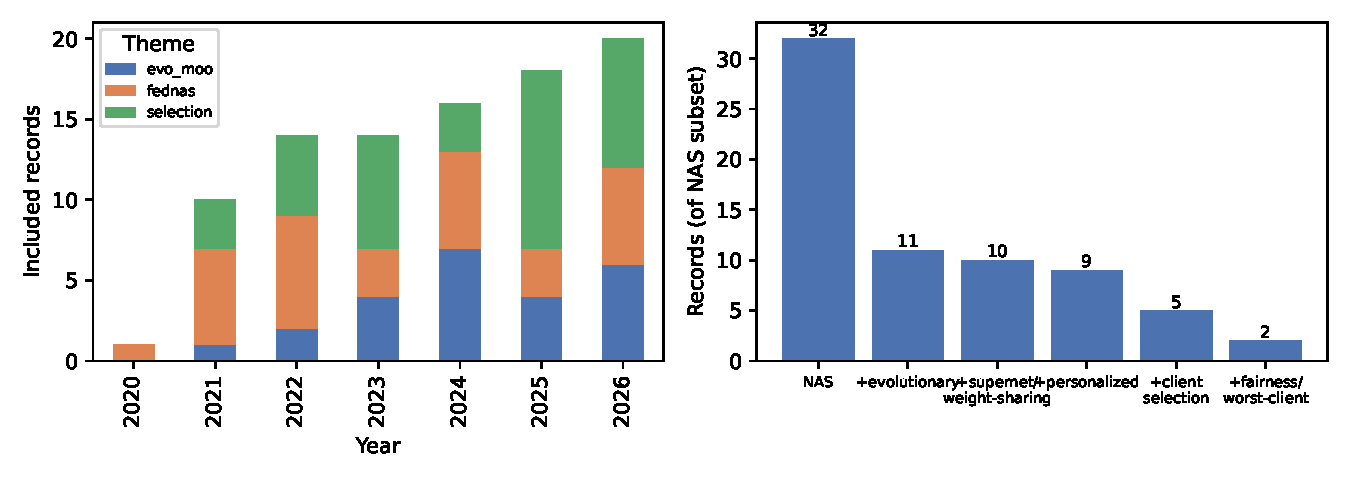
\includegraphics[width=\linewidth]{figures/corpus_overview.pdf}
\caption{Left: included records per year and theme. Right: among the \nnas{} NAS records, how many (abstract-coded) also involve each feature.}\label{fig:overview}\end{figure}

\subsection{RQ1: Federated NAS}
The foundational surveys and early systems frame FedNAS as the combination of NAS with FL's privacy and heterogeneity constraints \cite{zhu2021from,garg2020direct}. Four design families recur.

\textbf{Supernet and weight-sharing search.} Many systems search a weight-sharing supernet and extract sub-networks per device class, for example FedorAS \cite{dudziak2022fedoras}, supernet training under system heterogeneity \cite{kim2022supernet}, divide-and-conquer sampling \cite{venkatesha2023divideandconquer} and the recent Pareto-guided DeepFedNAS \cite{khan2026deepfednas}. Hyper-parameter tuning has been connected to weight-sharing as well \cite{khodak2021federated}, and FEATHERS searches architecture and hyper-parameters jointly with differential privacy \cite{seng2022feathers}.

\textbf{Resource-aware and cost-reducing search.} Yuan et al.\ decouple search from training and cut client cost through parallel candidate training on \emph{partial clients}, early dropping of weak candidates and dynamic round numbers \cite{yuan2022resourceaware}. Zhu and Jin's real-time evolutionary FedNAS uses a double-sampling scheme in which each individual transmits only a randomly sampled sub-model to randomly sampled clients \cite{zhu2021realtime}. Other work targets hierarchical search spaces \cite{liu2023finch}, energy \cite{wang2025energyfriendly}, carbon constraints \cite{patel2026designing} or heterogeneous deployment \cite{zhang2023enasfl,yu2022resourceaware}.

\textbf{Personalised and tailored architectures.} A large share searches \emph{different} architectures per client or cluster \cite{mushtaq2021spider,yan2024peaches,yang2025heterogeneityaware,zhang2022toward,yan2026pfedzkd} (\nnaspers{} NAS records mention personalisation). These address a different problem from a single deployable global model.

\textbf{Evolutionary and swarm search.} Only \nnasevo{} of \nnas{} NAS records use or discuss evolutionary/swarm search (including the survey \cite{zhu2021from}). Besides \cite{zhu2021realtime}, examples are a PSO-based multi-objective framework optimising accuracy and model complexity with clustered populations \cite{li2026multiobjective}, a multi-objective NAS for epistasis detection \cite{wu2024a}, GPT-4-assisted PSO \cite{wang2024federated}, an evolutionary search-space generator inside a DARTS-based robust FedNAS \cite{zhang2024privacypreserving}, and evolutionary search for one-shot personalised FL \cite{yan2026pfedzkd}.

Most FedNAS evaluations report accuracy together with resource or communication savings (\nnasres{} of \nnas{} abstracts mention resources, \nnasnoniid{} mention heterogeneity or non-IID data). Only \nnasfair{} NAS abstracts mention a fairness or consistency angle, and neither abstract describes a worst-client search objective.

\subsection{RQ2: Evolutionary and multi-objective optimisation in FL}
Two usage patterns dominate.

\textbf{Selection and resource scheduling per round.} \nevosel{} records use evolutionary or swarm algorithms to choose participants: GA-based client groups \cite{umar2026resilient,kang2023ga}, surrogate-assisted evolutionary subset search \cite{qiang2026evocsfl}, many-objective device selection and aggregation in vehicular networks \cite{wen2024a,cai2025a}, multi-criteria client deployment \cite{chahoud2023ondemandfl}, and comparisons of swarm algorithms \cite{khan2024swarm,rodrigues2026psobased}. Their fitness is a property of the FL training round (accuracy gain, latency, energy, coverage), not of a candidate architecture.

\textbf{Multi-objective FL parameter or hyper-parameter optimisation.} NSGA-III with hierarchical clustering optimises error rate, accuracy variance and communication cost on non-IID data \cite{zhong2022optimizing}; Pareto formulations balance utility, privacy and efficiency \cite{kang2024optimizing}, resource efficiency and convergence \cite{jung2024federated}, or heterogeneity and model size \cite{tursunboev2025multiobjective}; SecureBoost hyper-parameters are tuned with a multi-objective federated search \cite{ren2023secureboost}. A survey and taxonomy of multi-objective methods in FL is available \cite{hartmann2025multiobjective}.

\textbf{Gradient-based federated multi-objective learning.} A parallel strand treats \emph{clients} as objectives and applies multi-gradient descent with Pareto-stationarity \cite{askin2024federated,jiansheng2025federated,dehghanpour2026fedhv,guo2026fewformany}. Worst-client performance is an explicit objective in fairness-oriented formulations \cite{cui2021addressing}.

\subsection{RQ3: Similarity, divergence and clustering for participant selection}
Of \nseltotal{} records coded as selection/sampling, \nselsim{} use a similarity, divergence, gradient or clustering signal. The signals are:
\begin{itemize}
\item \emph{weight or update divergence}: weight divergence to identify non-IID degree \cite{zhang2021client}, divergence combined with loss \cite{guo2021wcl}, Euclidean distance of updates to the global model \cite{2025euclideanbased}, gradient projection \cite{na2025gpfl}, gradient-update-based heterogeneity \cite{balivada2026heterogeneityaware};
\item \emph{label or data similarity and clustering}: label-distribution clustering with equitable representation \cite{bhope2023flips,jimenezgutierrez2026fedlecc}, one-time clustering on learned features and stratified sampling \cite{abebe2023lefl}, similarity-metric clustering with one client per cluster \cite{fama2024measuring}, variance-reduction clustering \cite{shen2022fast}, group selection \cite{li2022data};
\item \emph{low-similarity or diverse sampling}: sampling that avoids redundant, similar updates \cite{kang2025lowsimilarity,liangyan2025pncspowernorm};
\item \emph{clustered FL}, which groups clients to train multiple models rather than to cut cost \cite{long2022multicenter,morafah2023flis,cheng2025snapcfl}.
\end{itemize}
Two orientations therefore co-exist: selecting \emph{diverse} (dissimilar) clients to cover the population, and selecting \emph{similar} clients or cluster representatives to avoid redundancy. We found no record in this corpus that directly compares the two orientations on the same budget. Equitable or fair selection is a distinct line \cite{jimenez2024submodular,arisdakessian2025towards,alsofyani2026a}, and surveys cover the area broadly \cite{smestad2023a,baker2025a,wijethilake2026federated,baduwal2026federated}. Reinforcement-learning selectors form another group (\nrlsel{} records) \cite{zhao2025fedppo}. In all of these, the quantity being optimised or accelerated is the \emph{training} of one FL model, not the screening of many architectures.

\subsection{RQ4: Intersections, fairness objectives and cost reporting}
Table~\ref{tab:gap} summarises the intersections. Using abstract coding followed by manual inspection of each non-zero intersection:
\begin{itemize}
\item \emph{NAS with participant subsampling for candidate evaluation}: two records, \cite{zhu2021realtime} (random clients per individual) and \cite{yuan2022resourceaware} (candidates evaluated on client groups). Full-text reading (Section~\ref{sec:fulltext}) shows that the first chooses clients at random and the second builds groups that balance data count and match the global label distribution; neither uses update similarity or dissimilarity, and neither optimises a worst-client objective.
\item \emph{NAS with cluster-based client grouping}: the keyword coding found \nnassim{} records, but manual reading found one: Finch divides clients into clusters by data distribution and allocates sub-networks sampled from a supernet to the clusters for parallel search \cite{liu2023finch}. The clusters speed up a supernet-based search; the abstract does not describe choosing a similarity- or dissimilarity-based subset of clients to evaluate each candidate.
\item \emph{Evolutionary NAS with client selection}: \nnasevosel{} coded record \cite{zhu2021realtime}.
\item \emph{Worst-client or fairness in the architecture-search objective}: not found among the NAS records.
\end{itemize}
Whether these studies report cost in a way that separates local trainings, probe/characterisation overhead, communication and wall-clock time cannot be judged from abstracts; the full-text assessment is left to future work.

\begin{table}[H]\centering\small
\caption{Coverage of intersections among the \nN{} included records (abstract-coded, then manually checked for the NAS rows).}\label{tab:gap}
\begin{tabular}{lr}\toprule
Combination & Records\\\midrule
FedNAS (all) & \nnas\\
\quad + evolutionary/swarm & \nnasevo\\
\quad + multi-objective & \nnasmoo\\
\quad + participant subsampling (manually verified) & 2\\
\quad + cluster-based client grouping (manually verified) & 1\\
\quad + fairness / worst-client objective & 0 (manual)\\
Evolutionary/swarm + client selection (no NAS) & \nevosel\\
Client selection + similarity/divergence/cluster & \nselsim\\
Client selection + fairness-oriented & \nselfair\\\bottomrule
\end{tabular}\end{table}


\section{Full-text appraisal of the closest studies}\label{sec:fulltext}
The abstract-level screening cannot tell how studies are evaluated. We therefore retrieved the open-access full text of the studies closest to the project (federated NAS with cost reduction or evolutionary search, plus the two most relevant participant-selection papers) and extracted, with keyword-located passages and targeted reading of method and experiment sections, the items in Table~\ref{tab:fulltext}. \textbf{This is a targeted extraction, not a close reading of every page.} Thirteen texts were obtained from arXiv; the Yuan et al.\ text is arXiv v5 of the same system as the published journal paper \cite{yuan2022resourceaware} (the journal text was not accessible, and the two are treated as one study). Finch \cite{liu2023finch} (paywalled), and \cite{li2026multiobjective,zhong2022optimizing} (publisher blocked automated access) could not be read in full and remain abstract-only; we did not try to circumvent access restrictions. ``None found'' means that keyword search of the text located no statement, so a statement present only in a figure or table could be missed. The structured extraction is in \texttt{fulltext/extraction.csv}.

\begin{landscape}
\begin{table}[p]\centering\scriptsize
\caption{Full-text extraction for the closest studies. Val/test = how validation and test data are used during search; Rep. = repeated runs reported.}\label{tab:fulltext}
\begin{tabular}{@{}p{2.5cm}p{4cm}p{3.6cm}p{4.4cm}p{1.9cm}p{3.1cm}p{3.1cm}@{}}\toprule
Study & Search / fitness & Data, heterogeneity & Clients used during search & Rep. & Val/test in search & Cost reported\\\midrule
Zhu \& Jin \cite{zhu2021realtime} & NSGA-II (pop.\ 10, 500 gen.) over sub-models of a master network; objectives: error, FLOPs & CIFAR-10; 10/20/50 clients; non-IID = 5 classes/client & Random disjoint clients per individual ($L=\lfloor m/N\rfloor$), each client used once per generation & none found & Objective is called ``test error''; no separate held-out split described & FLOPs; rounds; about 5$\times$ faster per round than offline evolutionary NAS\\
Yuan et al.\ \cite{yuan2022resourceaware} & Adapts a pre-trained CNN; early dropping; dynamic rounds & ImageNet (IID, 1\,500 clients); CelebA (non-IID, 9\,343 clients) & Clients partitioned into $K$ groups balanced in data count and in distance of group label distribution to the global one & none found & Clients split local data into train and validation & Client compute/communication; up to 200$\times$ lower than a straightforward federated NAS\\
FedorAS \cite{dudziak2022fedoras} & Supernet + NSGA-II per device tier (accuracy vs size) & CIFAR-10 (LDA $\alpha\in\{1000,1,0.1\}$), CIFAR-100, Speech Commands, Shakespeare & $k$ of $K$ clients per round in supernet training; Oort/PyramidFL as selection comparators & 3 repeats (random-search baseline only) & Centralised validation set from held-out client data; separate test & Random search at equal budget (about 40 full models) is worse by 0.25--12.8 pp\\
FEATHERS \cite{seng2022feathers} & DARTS-style supernet + bandit HPO with DP & Fashion-MNIST and others; 5/10/100 clients, IID and label-skew & Cross-silo: all clients & 5 repeats, mean $\pm$ SD & not described & Rounds (1\,500 in evaluation stage)\\
FedEx \cite{khodak2021federated} & Weight-sharing HPO vs random search and successive halving & Shakespeare, FEMNIST, CIFAR-10 & Fixed clients per round; noisy validation from few clients named a key challenge & 3 trials & Validation data split across devices & Communication rounds\\
DC-NAS \cite{venkatesha2023divideandconquer} & Supernet; diversified subnet sampling & CIFAR-10 (8 clients, $\alpha=0.5$), CIFAR-100, EMNIST, TinyImageNet & Subnets divided among clients per round & none found & Local train/val; held-out global test set & About 50\% fewer resources; vs random and Hadamard sampling\\
DFNAS \cite{garg2020direct} & Supernet (420 / 312 architectures) & CIFAR-10, CINIC-10; 8 clients non-IID & All clients & none found & Test accuracy vs rounds & Rounds vs FedAvg with fixed CNNs\\
DeepFedNAS$^{*}$ \cite{khan2026deepfednas} & Pareto-guided supernet; predictor-free search & CIFAR-10/100 ($K{=}20$), CINIC-10 ($K{=}100$); $\alpha=100$ main, 1 and 0.1 analysis & Fraction $C{=}0.4$ as reported & mean $\pm$ SD over 5 post-training search seeds & Validation split for checkpoints and search decisions & MACs; search time (about 20 s on CPU)\\
EvoCSFL$^{*}$ \cite{qiang2026evocsfl} & Surrogate-assisted evolutionary client-subset selection (no NAS) & Dirichlet; $K{=}10$ of $N{=}100$ per round & Evolved subset per round & none found & not described & 3.98 s overhead/round vs 9.2 min training\\
FLIPS \cite{bhope2023flips} & Label-distribution clustering for participant selection (no NAS) & $\alpha\in\{0.3,0.6\}$; 200 parties; 4 datasets & 15\% or 20\% of parties; every cluster represented & mean of 6 runs & Global test set (emulation) & Communication 20--60\% lower; rounds to target\\
FedSup \cite{kim2022supernet} & Federated supernet training & CIFAR-100; 100 clients; shards, Dirichlet & Participation ratio $R$ & none found & not described & Accuracy\\
SPIDER \cite{mushtaq2021spider} & Personalised architecture search & Dirichlet; 8 clients & All clients & none found & Per-client test accuracy on 20\% local hold-out & Model size\\\bottomrule
\multicolumn{7}{@{}l}{\scriptsize $^{*}$ preprint. The survey \cite{zhu2021from} was also retrieved and used for taxonomy only.}
\end{tabular}\end{table}
\end{landscape}

\subsection{Observations}
\begin{enumerate}
\item \textbf{Informed client groups for candidate evaluation exist, and the abstract-level result needs correcting.} Yuan et al.\ partition the available clients into groups and evaluate each candidate on one group, explicitly choosing groups so that their label distribution is close to the global one, because a random partition ``may lead to groups with biased data'' and make the search ``choose the wrong candidate'' \cite{yuan2022resourceaware}. This is distribution-aware participant choice for candidate evaluation, though it relies on clients uploading data-distribution information (a privacy trade-off) rather than update similarity or dissimilarity. Our abstract-level claim that such subsets were random or scheduled was therefore too strong; the corrected statement is in Section~\ref{sec:synthesis}.
\item \textbf{Noisy validation under partial participation is acknowledged but rarely measured.} FedEx identifies validation from a few clients per round as a noisy surrogate and shows that simple state-estimation fixes do not help \cite{khodak2021federated}; Yuan et al.\ motivate group balancing by the same risk. No study in the extracted set reports how often a subset-based ranking of candidates agrees with a full-participation ranking.
\item \textbf{Repeats are reported in a minority.} Repeated runs or seeds appear in FEATHERS (5), FedEx (3), FLIPS (6), DeepFedNAS (5 \emph{search} seeds after one training) and, for the random baseline only, FedorAS (3). For the others no statement was located by keyword search.
\item \textbf{Validation/test discipline varies.} Zhu and Jin optimise a quantity called test error and report the same quantity as test accuracy \cite{zhu2021realtime}; FedorAS uses a centralised validation set assembled from held-out client data \cite{dudziak2022fedoras}; DC-NAS and FLIPS evaluate on a global test set \cite{venkatesha2023divideandconquer,bhope2023flips}. These server-side pooled sets are convenient but depart from strict client-side evaluation. The project's per-client validation and test splits are the stricter choice.
\item \textbf{Heterogeneity levels are mostly mild.} Main comparisons use $\alpha=100$ \cite{khan2026deepfednas}, 5 classes per client \cite{zhu2021realtime}, or $\alpha=0.5$ \cite{venkatesha2023divideandconquer}; severe settings ($\alpha=0.1$) appear in robustness analyses \cite{dudziak2022fedoras,khan2026deepfednas}.
\item \textbf{Worst-client behaviour and hypervolume are absent from the empirical sections.} Only SPIDER plots per-client accuracy \cite{mushtaq2021spider}. No extracted study reports hypervolume or a worst-client metric as a search outcome, although two use Pareto fronts for accuracy versus size \cite{zhu2021realtime,dudziak2022fedoras}.
\item \textbf{Random baselines are informative.} FedorAS shows random search at equal budget to be worse by up to 12.8 pp \cite{dudziak2022fedoras}, in a much larger search space than the project's, which may explain why random search is competitive in the project's small MLP space.
\end{enumerate}

\section{Synthesis and research gaps}\label{sec:synthesis}
\begin{enumerate}
\item \textbf{Single global architecture under FedAvg is under-represented.} The dominant FedNAS framing is personalised or per-device-class architecture. Work that evaluates one architecture as a standard FedAvg-trained global model, with accuracy \emph{across clients} as the fitness, is rare in this corpus.
\item \textbf{Evaluation-cost reduction relies on random or label-distribution-based subsets.} The two NAS records that evaluate candidates on a subset of clients choose it at random \cite{zhu2021realtime} or by matching the group label distribution to the global one \cite{yuan2022resourceaware}. Whether choices based on the similarity or dissimilarity of client \emph{updates} improve over random or label-distribution-matched subsets at equal cost has, in this corpus, not been tested for NAS.
\item \textbf{Selection research optimises training, not search.} Divergence- and cluster-based selectors are evaluated on convergence speed and final accuracy of one model; the noisy, low-fidelity fitness that NAS needs (few rounds, few epochs) is a different regime.
\item \textbf{Worst-client objectives live in gradient-based federated multi-objective learning} rather than in evolutionary architecture search, so Pareto-front quality indicators (e.g.\ hypervolume) are not comparable across the two literatures.
\item \textbf{Methodological rigour is hard to assess.} Abstract-level evidence does not allow us to say how many studies use paired seeds, separate validation from test during search, or report cost components separately; these should be extracted from full texts.
\end{enumerate}

\subsection*{Implications for the EvoFederated study}
These gaps suggest specific comparators and checks for the present project: (i) random subsampling of clients per candidate \cite{zhu2021realtime} is the natural baseline for similarity/dissimilarity-based participant choice and is already included as \emph{random-$k$}, while the label-distribution-matched grouping of \cite{yuan2022resourceaware} is a stronger baseline that is missing (it needs distribution information that the update-based probe does not use); (ii) early dropping of weak candidates \cite{yuan2022resourceaware} is a cost lever orthogonal to participant choice and is not yet evaluated; (iii) a many-objective formulation with one objective per client is mirrored in \cite{zhong2022optimizing}, supporting the NSGA-III/MOEA/D comparison; (iv) second-dataset, multi-$\alpha$ evaluation and paired-seed reporting are not guaranteed by the surveyed literature and must be supplied by the study itself. This review does not show that any of the surveyed approaches outperforms another; it only locates the unexplored combination.

\section{Threats to validity}\label{sec:threats}
\begin{itemize}
\item \textbf{Single source and depth limit.} Only OpenAlex was queried, and only the top 200 records per query. Relevant items outside these ranks, or indexed elsewhere (IEEE Xplore, ACM DL, Scopus, Semantic Scholar, arXiv), may be missed.
\item \textbf{Single reviewer, abstract-level screening; partial full-text coverage.} Only 13 studies were extracted from full text, with keyword-located passages rather than complete close reading; the journal texts of Yuan et al.\ and Finch were not accessible. No dual screening or inter-rater agreement; keyword coding is approximate and may over- or under-count (e.g.\ ``sampling'' also matches model sampling).
\item \textbf{Keyword pre-filter.} Records whose abstracts lack the terms in \texttt{screen.py} were dropped before manual review.
\item \textbf{Publication status.} \npre{} of \nN{} records are preprints; several are 2026 and not peer-reviewed.
\item \textbf{Date coverage.} Publications before 2019 were excluded, so classic work on federated optimisation and on evolutionary NAS in centralised settings is outside scope.
\item \textbf{No claim of exhaustiveness.} ``No record found'' statements refer to this corpus only.
\end{itemize}

\section{Conclusion}
FedNAS, evolutionary/multi-objective FL and participant selection are each active, but their intersection is thin. In the \nN{} included records, evaluation cost in NAS is reduced by random or label-distribution-matched client subsets, update-similarity and divergence signals are used to speed up training rather than architecture search (label-distribution matching has been used for candidate evaluation), and worst-client behaviour is optimised by gradient-based methods rather than evolutionary NAS. A reproducible study of informed versus random participant choice for architecture evaluation, with a mean/worst-client objective and explicit cost accounting, is therefore a well-defined contribution, provided it is evaluated with adequate seeds, datasets and heterogeneity levels.

\appendix
\section{Included records}
\begin{longtable}{p{0.27\linewidth}rcl cccccc}
\caption{Included records with abstract-coded attributes (approximate; see Section~\ref{sec:methods}). NAS: architecture search; Evo: evolutionary/swarm; MOO: multi-/many-objective; Sel: client/participant selection or sampling; Sim: similarity/clustering/divergence; Fair: fairness/worst-client.}\label{tab:included}\\
\toprule
Record & Year & Peer & Theme & NAS & Evo & MOO & Sel & Sim & Fair\\
\midrule\endfirsthead
\toprule Record & Year & Peer & Theme & NAS & Evo & MOO & Sel & Sim & Fair\\\midrule\endhead
\cite{cui2021addressing} & 2021 &  & Evo/MOO &  &  & \checkmark &  & \checkmark & \checkmark\\
\cite{zhong2022optimizing} & 2022 & \checkmark & Evo/MOO &  & \checkmark & \checkmark &  & \checkmark & \\
\cite{2022adaptive} & 2022 & \checkmark & Evo/MOO &  & \checkmark &  & \checkmark &  & \\
\cite{xu2023a} & 2023 & \checkmark & Evo/MOO &  &  & \checkmark & \checkmark &  & \\
\cite{chahoud2023ondemandfl} & 2023 & \checkmark & Evo/MOO &  & \checkmark & \checkmark & \checkmark &  & \\
\cite{kang2023ga} & 2023 & \checkmark & Evo/MOO &  & \checkmark &  & \checkmark &  & \\
\cite{ren2023secureboost} & 2023 &  & Evo/MOO &  &  & \checkmark & \checkmark & \checkmark & \\
\cite{jung2024federated} & 2024 & \checkmark & Evo/MOO &  &  & \checkmark & \checkmark & \checkmark & \\
\cite{wen2024a} & 2024 & \checkmark & Evo/MOO &  & \checkmark & \checkmark & \checkmark &  & \\
\cite{yu2024towards} & 2024 & \checkmark & Evo/MOO &  &  & \checkmark &  &  & \checkmark\\
\cite{kang2024optimizing} & 2024 & \checkmark & Evo/MOO &  & \checkmark & \checkmark &  &  & \checkmark\\
\cite{cha2024multiobjective} & 2024 & \checkmark & Evo/MOO &  &  & \checkmark & \checkmark &  & \\
\cite{khan2024swarm} & 2024 &  & Evo/MOO &  & \checkmark &  & \checkmark &  & \\
\cite{askin2024federated} & 2024 &  & Evo/MOO &  &  & \checkmark &  & \checkmark & \\
\cite{cai2025a} & 2025 & \checkmark & Evo/MOO &  & \checkmark & \checkmark & \checkmark &  & \checkmark\\
\cite{tursunboev2025multiobjective} & 2025 & \checkmark & Evo/MOO &  & \checkmark & \checkmark & \checkmark & \checkmark & \\
\cite{hartmann2025multiobjective} & 2025 &  & Evo/MOO &  &  & \checkmark &  &  & \checkmark\\
\cite{jiansheng2025federated} & 2025 &  & Evo/MOO &  &  & \checkmark &  & \checkmark & \checkmark\\
\cite{umar2026resilient} & 2026 & \checkmark & Evo/MOO &  & \checkmark &  & \checkmark & \checkmark & \\
\cite{guo2026fewformany} & 2026 &  & Evo/MOO &  &  & \checkmark &  & \checkmark & \\
\cite{qiang2026evocsfl} & 2026 &  & Evo/MOO &  & \checkmark &  & \checkmark &  & \\
\cite{dehghanpour2026fedhv} & 2026 &  & Evo/MOO &  &  & \checkmark &  & \checkmark & \\
\cite{geng2026historyaware} & 2026 & \checkmark & Evo/MOO &  &  & \checkmark & \checkmark &  & \checkmark\\
\cite{rodrigues2026psobased} & 2026 & \checkmark & Evo/MOO &  & \checkmark &  & \checkmark &  & \\
\cite{garg2020direct} & 2020 &  & FedNAS & \checkmark &  &  &  &  & \\
\cite{zhu2021from} & 2021 & \checkmark & FedNAS & \checkmark & \checkmark & \checkmark &  & \checkmark & \\
\cite{zhu2021realtime} & 2021 & \checkmark & FedNAS & \checkmark & \checkmark &  & \checkmark &  & \\
\cite{wang2021flagcns} & 2021 &  & FedNAS & \checkmark & \checkmark &  &  &  & \\
\cite{mushtaq2021spider} & 2021 &  & FedNAS & \checkmark &  &  &  &  & \\
\cite{khodak2021federated} & 2021 &  & FedNAS & \checkmark &  &  &  &  & \\
\cite{liang2021selfsupervised} & 2021 &  & FedNAS & \checkmark &  &  & \checkmark &  & \\
\cite{zhang2022toward} & 2022 & \checkmark & FedNAS & \checkmark &  &  &  & \checkmark & \\
\cite{kim2022supernet} & 2022 &  & FedNAS & \checkmark &  &  &  &  & \\
\cite{liu2022federated} & 2022 & \checkmark & FedNAS & \checkmark & \checkmark & \checkmark &  &  & \\
\cite{yuan2022resourceaware} & 2022 & \checkmark & FedNAS & \checkmark &  &  &  &  & \\
\cite{yu2022resourceaware} & 2022 &  & FedNAS & \checkmark &  &  & \checkmark &  & \\
\cite{dudziak2022fedoras} & 2022 &  & FedNAS & \checkmark &  &  &  &  & \\
\cite{seng2022feathers} & 2022 &  & FedNAS & \checkmark &  &  &  &  & \\
\cite{liu2023finch} & 2023 & \checkmark & FedNAS & \checkmark &  &  &  & \checkmark & \\
\cite{zhang2023enasfl} & 2023 & \checkmark & FedNAS & \checkmark &  &  &  &  & \\
\cite{venkatesha2023divideandconquer} & 2023 &  & FedNAS & \checkmark &  &  & \checkmark &  & \\
\cite{wu2024a} & 2024 & \checkmark & FedNAS & \checkmark & \checkmark & \checkmark &  &  & \\
\cite{yan2024peaches} & 2024 & \checkmark & FedNAS & \checkmark &  &  &  &  & \\
\cite{wu2024generalizable} & 2024 & \checkmark & FedNAS & \checkmark &  &  &  &  & \checkmark\\
\cite{wang2024federated} & 2024 & \checkmark & FedNAS & \checkmark & \checkmark &  &  &  & \\
\cite{zhang2024privacypreserving} & 2024 & \checkmark & FedNAS & \checkmark & \checkmark &  &  &  & \\
\cite{pengyu2024personalized} & 2024 &  & FedNAS & \checkmark &  &  &  &  & \\
\cite{chen2025fedregnas} & 2025 & \checkmark & FedNAS & \checkmark &  &  &  & \checkmark & \\
\cite{yang2025heterogeneityaware} & 2025 & \checkmark & FedNAS & \checkmark &  &  &  &  & \\
\cite{wang2025energyfriendly} & 2025 & \checkmark & FedNAS & \checkmark & \checkmark &  &  &  & \\
\cite{li2026multiobjective} & 2026 & \checkmark & FedNAS & \checkmark & \checkmark & \checkmark &  & \checkmark & \\
\cite{yan2026pfedzkd} & 2026 & \checkmark & FedNAS & \checkmark & \checkmark &  &  & \checkmark & \checkmark\\
\cite{medjadji2026optimized} & 2026 &  & FedNAS & \checkmark &  & \checkmark &  &  & \\
\cite{khan2026deepfednas} & 2026 &  & FedNAS & \checkmark &  & \checkmark & \checkmark &  & \\
\cite{patel2026designing} & 2026 &  & FedNAS & \checkmark & \checkmark &  &  &  & \\
\cite{henze2026neural} & 2026 &  & FedNAS & \checkmark &  &  &  &  & \\
\cite{acar2021federated} & 2021 &  & Selection &  &  &  &  & \checkmark & \\
\cite{zhang2021client} & 2021 & \checkmark & Selection &  &  &  & \checkmark & \checkmark & \\
\cite{guo2021wcl} & 2021 & \checkmark & Selection &  &  &  & \checkmark & \checkmark & \\
\cite{li2022data} & 2022 & \checkmark & Selection &  &  &  & \checkmark & \checkmark & \\
\cite{long2022multicenter} & 2022 & \checkmark & Selection &  &  &  &  & \checkmark & \\
\cite{huang2022stochastic} & 2022 & \checkmark & Selection &  &  &  & \checkmark &  & \checkmark\\
\cite{jeong2022a} & 2022 & \checkmark & Selection &  &  &  & \checkmark & \checkmark & \checkmark\\
\cite{shen2022fast} & 2022 &  & Selection &  &  &  & \checkmark & \checkmark & \\
\cite{dang2023hybrid} & 2023 & \checkmark & Selection &  &  & \checkmark & \checkmark &  & \\
\cite{morafah2023flis} & 2023 & \checkmark & Selection &  &  &  &  & \checkmark & \\
\cite{smestad2023a} & 2023 &  & Selection &  &  &  & \checkmark &  & \checkmark\\
\cite{chen2023optimization} & 2023 &  & Selection &  &  &  & \checkmark & \checkmark & \\
\cite{bhope2023flips} & 2023 &  & Selection &  &  &  & \checkmark & \checkmark & \checkmark\\
\cite{zhang2023multicriteria} & 2023 &  & Selection &  &  &  & \checkmark &  & \checkmark\\
\cite{abebe2023lefl} & 2023 &  & Selection &  &  &  & \checkmark & \checkmark & \\
\cite{moon2024client} & 2024 & \checkmark & Selection &  &  & \checkmark & \checkmark &  & \\
\cite{jimenez2024submodular} & 2024 &  & Selection &  &  &  & \checkmark & \checkmark & \checkmark\\
\cite{fama2024measuring} & 2024 &  & Selection &  &  &  & \checkmark & \checkmark & \\
\cite{baker2025a} & 2025 & \checkmark & Selection &  &  &  & \checkmark & \checkmark & \checkmark\\
\cite{2025euclideanbased} & 2025 & \checkmark & Selection &  &  &  & \checkmark & \checkmark & \\
\cite{kang2025lowsimilarity} & 2025 & \checkmark & Selection &  &  &  & \checkmark & \checkmark & \checkmark\\
\cite{cheng2025snapcfl} & 2025 & \checkmark & Selection &  &  &  & \checkmark & \checkmark & \\
\cite{ma2025the} & 2025 & \checkmark & Selection &  &  &  & \checkmark & \checkmark & \\
\cite{zhao2025fedppo} & 2025 & \checkmark & Selection &  &  &  & \checkmark & \checkmark & \\
\cite{ghazi2025federated} & 2025 & \checkmark & Selection &  &  &  & \checkmark &  & \checkmark\\
\cite{peng2025federated} & 2025 & \checkmark & Selection &  & \checkmark &  & \checkmark & \checkmark & \\
\cite{na2025gpfl} & 2025 & \checkmark & Selection &  &  &  & \checkmark & \checkmark & \\
\cite{arisdakessian2025towards} & 2025 & \checkmark & Selection &  &  &  & \checkmark &  & \checkmark\\
\cite{liangyan2025pncspowernorm} & 2025 &  & Selection &  &  &  & \checkmark & \checkmark & \\
\cite{balivada2026heterogeneityaware} & 2026 &  & Selection &  &  &  & \checkmark & \checkmark & \\
\cite{baduwal2026federated} & 2026 & \checkmark & Selection &  &  &  & \checkmark &  & \checkmark\\
\cite{abboud2026feddcsrw} & 2026 & \checkmark & Selection &  &  &  & \checkmark & \checkmark & \\
\cite{zhao2026a} & 2026 & \checkmark & Selection &  &  &  & \checkmark & \checkmark & \\
\cite{jimenezgutierrez2026fedlecc} & 2026 &  & Selection &  &  &  & \checkmark & \checkmark & \\
\cite{alsofyani2026a} & 2026 & \checkmark & Selection &  &  &  & \checkmark &  & \checkmark\\
\cite{wijethilake2026federated} & 2026 & \checkmark & Selection &  &  &  & \checkmark &  & \checkmark\\
\cite{zhang2026prototype} & 2026 & \checkmark & Selection &  &  &  & \checkmark & \checkmark & \\
\bottomrule
\end{longtable}


\bibliographystyle{unsrt}
\bibliography{references_included,background}
\end{document}
